\documentclass{assignmeownt}

\coursenumber{CH 420}
\coursetitle{Understanding Advanced Molecular Simulation}
\title{Block 2}
\author{Qianjun Xu}
\date{}

\begin{document}
\maketitle
\thispagestyle{firststyle}
\bigskip

\question{Calculation of $\pi$}

\questionpart{How can $\pi$ be calculated from the fraction of points that fall in the circle? Complete
the small Monte Carlo program to calculate $\pi$ using this method.}

We know that the area of a square of length $l$ is $l^2$ and the area of a circle of diameter $d$ is $\frac{\pi d^2}{4}$. Thus the probability of a randomly dropped point fall in the circle is

$$P=\frac{\pi d^2}{4 l^2}=\frac{\pi}{4 ratio^2}$$


By calculate the ratio of the number of points fall in the circle and the number of the whole points, we can calculate the $\pi$ and here is the program (Figure \ref{fig:calculate_pi}).\\

\questionpart{How would you expect that the accuracy of the result depends on the ratio $l/d$ and
the number of generated coordinates?}

\questionpart{Derive a formula to calculate the relative standard deviation of the estimate of $\pi$.}

This algorithm can be described by a binomial distribution $B(N, P)$, whose mean is $NP$ and the variance is $NP(1-P)$. If we denote the experiment result as $b_i$, what we are interested in are
$$
\bar{b}=\frac{1}{N}\sum_{i=1}^N b_i = P
$$
$$
\sigma^2(\bar{b})=\frac{1}{N^2}\sum_{i=1}^N b_i^2 - \bar{b}^2 = \frac{P(1-P)}{N}
$$
And thus the standard deviation of the estimate of $\pi$ is $\sqrt{\sigma^2(\bar{b})}=\sqrt{\frac{P(1-P)}{N}}$. We here use the relative standard deviation to study the accuracy of the result. 
$$
\frac{\sigma}{\bar{b}}=\sqrt{\frac{1-P}{NP}}=\sqrt{\frac{4ratio^2}{N\pi}-\frac{1}{N}}
$$

From this we can see that the accuracy of the result depends on the ratio $l/d$ and the number of generated coordinates. The smaller the ratio is (but it must be at least 1), and the larger the number of generated coordinates is, the more accurate the result is.

\questionpart{Is it a good idea to calculate many decimals of $\pi$ using this method?}

This method can provide us with a approximation of the $\pi$, but is not a good way to calculate the $\pi$ accurately, because its value converge to the exact value of $\pi$ in probability. That is to say, no matter how many points we drop, it is still possible that there is a large deviation from the exact value.


\question{The Photon Gas}
\begin{figure}
    \centering
    \includegraphics[width=0.5\linewidth]{../block2/1-CalculationOfPi/Results/mc.png}
    \caption{The program of calculating $\pi$.}
    \label{fig:calculate_pi}
  \end{figure}


\questionpart{How can this scheme obey detailed balance when $n_j = 0$?}
To obey detaied balance when $n_j=0$, if the trail move is to decrease $n_j$ by 1, we cancel this move. Thus the probability for $0$ to move to $-1$ and move from $-1$ are both $0$.

\questionpart{Is the algorithm still correct when trial moves are performed that change $n_j$ with a
random integer from the interval [-5, 5]? What happens when only trial moves are
performed that change $n_j$ with either -3 or +3?}
The algorithm is correct when trial moves are performed that change $n_j$ with a random integer from the interval [-5, 5]. It however fails when only trial moves are performed that change $n_j$ with either -3 or +3, beacuse in this case, the prior probability $\alpha[0\rightarrow 1]\neq\alpha[1\rightarrow 0]=0$.

\questionpart{Assume that $N = 1$ and $\epsilon_j=\epsilon$. Use the small Monte Carlo program and the "run\_auto" script to calculate $\langle  n_j \rangle$ as a function of $\beta\epsilon$. Compare your result with the analytical solution.}

When we use the standard method, the result agrees with the analytical solution. (Figure \ref{fig:energy_as_function_of_beta}).

\begin{figure}
    \centering
    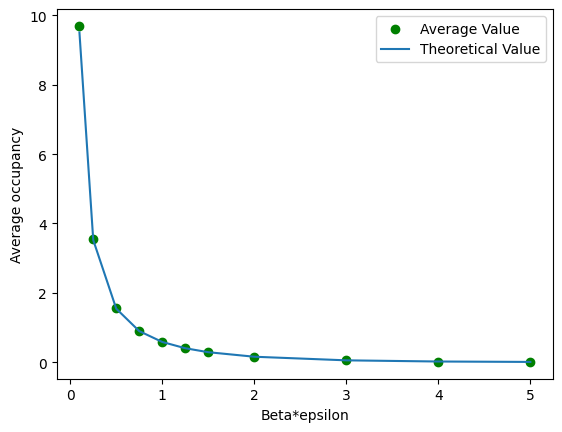
\includegraphics[width=0.5\linewidth]{../block2/2-PhotonGas/Results/correct.png}
    \caption{$\left< n_j \right> $ as a function of $\beta \epsilon$.}
    \label{fig:energy_as_function_of_beta}
  \end{figure}

\questionpart{Modify the program in such a way that the averages are updated only after an
accepted trial move. Why does this lead to erroneous results? At which values of $\beta$
does this error become more pronounced?}
The modified program is shown in Figure \ref{fig:modify_photon}. The erroneous results is more pronounced at larger values of $\beta$, that is to say, at lower temperature (Figure \ref{fig:modify_photon_result}).
\begin{figure}
    \centering
    \includegraphics[width=0.5\linewidth]{../block2/2-PhotonGas/Results/modify.png}
    \caption{The modified program of producing wrong result.}
    \label{fig:modify_photon}
\end{figure}

\begin{figure}
    \centering
    \includegraphics[width=0.5\linewidth]{../block2/2-PhotonGas/Results/error.png}
    \caption{Wrong result of the modified program.}
    \label{fig:modify_photon_result}
\end{figure}


\questionpart{Modify the program in such a way that the distribution of $n_j$ is calculated as well.
Compare this distribution with the analytical distribution}
Figure \ref{fig:record_distribution_of_nj} is the modified program. The following plot (Figure \ref{fig:distribution_of_nj}) is at $\beta=0.10$. The simulation result agrees well with the theory.

\begin{figure}
    \centering
    \includegraphics[width=0.5\linewidth]{../block2/2-PhotonGas/Results/record_distribution.png}
    \caption{Recording the distribution of $n_j$.}
    \label{fig:record_distribution_of_nj}
\end{figure}

\begin{figure}
    \centering
    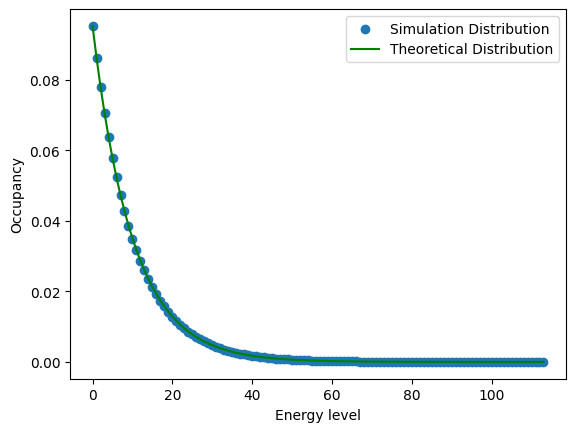
\includegraphics[width=0.5\linewidth]{../block2/2-PhotonGas/Results/distribution.png}
    \caption{The distribution of $n_j$ at $\beta=0.10$.}
    \label{fig:distribution_of_nj}
\end{figure}

\bigskip

\question{MC of a Lennard-Jones System}

\questionpart{In the present code, the pressure of the system is not calculated. Modify the code in such a way that the average pressure can be calculated. You will only have to make some modifications in the subroutine \textit{energy.c} to calculate the virial. Using this quantity, the pressure will then be calculated automatically.}
The modification is shown in Figure \ref{fig:energy_md}.

\begin{figure}
    \centering
    \includegraphics[width=0.5\linewidth]{../block2/3-MCLennardJones/Results/calc_energy.png}
    \caption{The modification for calculating the pressure.}
    \label{fig:energy_md}
\end{figure}

\questionpart{Perform a simulation at $T = 2.0$ and various densities. Up to which density does the ideal gas law hold?}
Below is the table (Table \ref{tab:ideal_gas}) and figure (Figure \ref{fig:ideal_gas}) for the pressure versus density at $T=2$. It can be seen that the ideal gas law holds at $\rho \in [0.1,\ 0.4]$.
\begin{table}[]
    \centering
    \caption[]{Pressure versus density at $T=2$.}
    
    \begin{tabular}{@{}cc@{}}
    \toprule
    Density & Pressure \\ 
    \midrule
    0.1     & 0.178    \\
    0.2     & 0.331    \\
    0.3     & 0.485    \\
    0.4     & 0.694    \\
    0.5     & 1.072    \\
    0.6     & 1.760    \\
    0.7     & 2.982   \\
    0.8     & 5.398   \\
    0.9     & 9.148   \\
    1.0     & 15.12   \\
    1.2     & 39.84   \\
    1.4     & 95.92   \\
    \bottomrule
    \end{tabular}
    \label{tab:ideal_gas}
\end{table}

\begin{figure}
    \centering
    \includegraphics[width=0.5\linewidth]{../block2/3-MCLennardJones/Results/pd.png}
    \caption{The distribution of $n_j$ at $\beta=0.10$.}
    \label{fig:ideal_gas}
\end{figure}

\questionpart{The program produces a sequence of snapshots of the state of the system. Try to visualise these snapshots using the program \textit{vmd}.}

Figure \ref{fig:snapshot} is the snapshot of the state of the system.

\begin{figure}
    \centering
    \includegraphics[width=0.5\linewidth]{../block2/3-MCLennardJones/Results/snapshot.jpg}
    \caption{The snapshot of the state of the system.}
    \label{fig:snapshot}
\end{figure}

\questionpart{Derive a formula for the dimensionless heat capacity. Modify the program (only in mc\_nvt.c) in such a way that $C_V$ is calculated.}
Figure \ref{fig:calc_cv} is the calculation of the heat capacity.

\begin{figure}
    \centering
    \includegraphics[width=0.6\linewidth]{../block2/3-MCLennardJones/Results/calc_cv.png}
    \caption{The calculation of the $C_v$.}
    \label{fig:calc_cv}
\end{figure}


The heat capacity $C_V=\frac{\left<U^2\right>-\left<U\right>^2}{Nk_BT^2}$ has a dimension of $J/K$. Thus, to make it a dimensionless, we can simply divide it by $k_B$:
$$C_V^*=\frac{\left<U^2\right>-\left<U\right>^2}{Nk_B^2T^2}=\frac{\left<U^2\right>-\left<U\right>^2}{N}\beta^2$$

\questionpart{Instead of performing a trial move in which only one particle is displaced, one
can do a trial move in which all particles are displaced. Compare the maximum displacements of these moves when 50\% of all displacements are accepted.}
\begin{figure}
    \centering
    \includegraphics[width=0.5\linewidth]{../block2/3-MCLennardJones/Results/move_system.png}
    \caption{The algorithm of moving the whole system.}
    \label{fig:move_system}
\end{figure}

Figure \ref{fig:move_system} is the algorithm of moving the whole system. The maximal displacement of moving a single particle is $0.20$. For moving all particles, the maximal displacement is $0.05$. ($T=1.0,\ \rho=0.1$) Because the maximal displacement of moving a single particle is larger, the simulation is more efficient.

\questionpart{Instead of using a uniformly distributed displacement, one can also use a Gaussian
displacement. Does this increase the efficiency of the simulation?}
A larger displacement is the core of sampling the system. The Gaussian distribution gives more smaller displacements while reduces the possibility of lager displacements. Thus the simulation might be less efficient.

\bigskip

\question{MD of a Lennard-Jones System}

\questionpart{Find the three errors in the code.}
Two errors are found in \textit{integrate.c} and one is found in \textit{force.c} (Figure \ref{fig:errors}).
\begin{figure}
    \centering
    \begin{subfigure}[b]{0.4\textwidth}
        \centering
        \includegraphics[width=\linewidth]{../block2/4-MDLennarJones/Results/error1.png}
        \caption{One error in \textit{integrate.c} in the calculation of the degree of freedom.}
    \end{subfigure}
    \begin{subfigure}[b]{0.4\textwidth}
        \centering
        \includegraphics[width=\linewidth]{../block2/4-MDLennarJones/Results/error2.png}
        \caption{The other error in \textit{integrate.c} also in the calculation of the degree of freedom.}
    \end{subfigure}
    \begin{subfigure}[b]{0.4\textwidth}
        \centering
        \includegraphics[width=\linewidth]{../block2/4-MDLennarJones/Results/error3.png}
        \caption{One error in \textit{force.c} in the calculation of the force.}
    \end{subfigure}
       \caption{The three errors.}
       \label{fig:errors}
  \end{figure}

\questionpart{How is the temperature controlled in this program? What does it mean to "control the temperature": after all, in a simulation at constant NVE it is the total energy of the system that should be constant, whilst the temperature fluctuates.}

During the initialization phase, the temperature is controlled by multiply the calculated velocity with a factor
$$ c = \sqrt{\frac{T_{expectation}}{\frac{\sum_{i=1}^N mv_{\alpha,\ i}^2(t)}{N_f}}}=\sqrt{\frac{T_{expectation}(3N-4)}{\sum_{i=1}^N mv_{\alpha,\ i}^2(t)}} $$

This scaling factor is defined based on the relationship
$$\left<v_\alpha^2\right>=k_BT/m$$
which describes the relationship between the kinetic energy and the instantaneous temperature. When performing the simulation, the instantanuous temperature sometimes deviates from the temperature we expect.
$$ T/T_{expectation}=\frac{m\left<v_\alpha^2\right>}{k_BT_{expectation}}$$

To tune the ratio to be 1, a scaling can be performed on the velocity
$$\frac{m\left<(cv_\alpha)^2\right>}{k_BT_{expectation}}=1$$
which leads to
$$c=\sqrt{\frac{k_BT_{expectation}}{m\left<v_\alpha^2\right>}}$$
and the expectation of the squared velocity is defined by
$$\left<v_\alpha^2\right>=\frac{\sum_{i=1}^{N}v_{\alpha,\ i}^2(t)}{N_f}=\frac{v_{\alpha,\ i}^2(t)}{3N-4}$$
This is how the first equation comes. Through this we can see the control over the temperature is actually a control of the kinetic energy. This helps us relax our initial structure, which might be unreasonable at first and leads to a blow up to the simulation system, and a sufficient equibilirium can help avoid this. After passing the first initialization steps, we no longer need this scaling anymore.

\questionpart{How does the time step for a given energy drift change with the temperature and density?}

From the Figure \ref{fig:drift_ts}, it can be seen that the drift of total energy increases with the length of the time step.

\begin{figure}
    \centering
    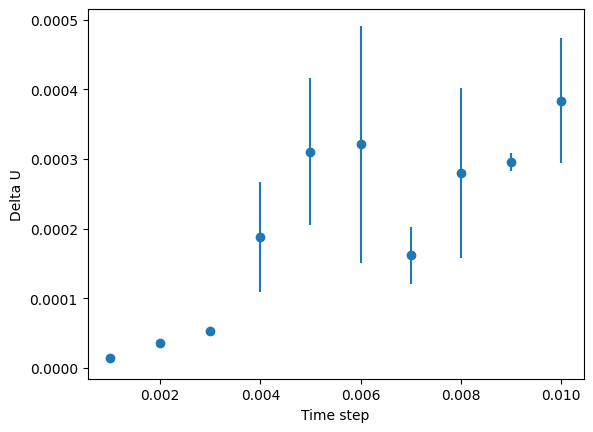
\includegraphics[width=0.5\linewidth]{../block2/4-MDLennarJones/Results/drift_ts.png}
    \caption{The drift of the total energy versus the length of time step.}
    \label{fig:drift_ts}
\end{figure}

Additionally, for a given energy drift, the higher the temperature and density are, the smaller the time step is.

\questionpart{As you might have noticed in the code, the implementation of the periodic boundary conditions is often done as ibox is used instead of 1/box. Why would one do this?}
Because it is more time efficient to calculate the result of $1 / box$ and store it, instead of calculate it every time. However, this performance improvement might be very small. For me, I would prefer to use $1 / box$ for the readablity of the code.

\questionpart{Modify the program in such a way that the self-diffusion coefficient can be calculated using both methods. Only modifications in subroutine sample\_diff.c are needed. It is not a good idea (although not wrong) to take every time step as a new time origin for the calculation of the VACF and of the mean-squared displacement. Explain. What is the unit of D in SI units? How can one transform D into dimensionless units?}

The implementation of the periodic boundry conditions (PBC) is to enable one to simulate a infinitly large system with countable atoms. The update of the coordinates of atoms out of the PBC box is necessary because the interactions between the atoms need to be calculated correctly.

To take every time step as a new time origin does increase the available data for calculate the VACF and the mean-squared displacement, while it is not efficient in terms of sampling. Whatsmore, when we have a very long trajectory, the calculation of the VACF and the mean-squared displacement is very expensive.

The modification of the program is shown in Figure \ref{fig:diffusion}.

\begin{figure}
    \centering
    \includegraphics[width=1.0\linewidth]{../block2/4-MDLennarJones/Results/modifiy.png}
    \caption{The calculation of the self-diffusion coefficient.}
    \label{fig:diffusion}
\end{figure}

The unit of $D$ in SI units is $m^2/s$. According to [Naghizadeh, 1962](https://doi.org/10.1063/1.1732357), if atoms interact pairwise with a two parameter potention, the reduced diffusion coefficient can be defined as
$$\tilde{D}=(m/\epsilon\sigma^2)^{1/2}D$$
where $m$ is the mass of the particle, $\epsilon$ is the depth of the potential well and $\sigma$ is a length related to the size of the particle.

\questionpart{For Lennard-Jones liquids, Naghizadeh and Rice report the following equation for the self-diffusion coefficient. Try to confirm this equation with simulations.}

Simulations are done to see if the equation can be got from simulation. Here I calculate the relative deviation of the self-diffusion coefficient.
$$
\frac{\tilde{D}_{simulation}-\tilde{D}_{equation}}{\tilde{D}_{simulation}}
$$
and plot the result in Figure \ref{fig:devi}. It can be seen that the equation can only be confirmed in low temperature and low presure area.

\begin{figure}
    \centering
    \includegraphics[width=0.5\linewidth]{../block2/4-MDLennarJones/Results/equation.png}
    \caption{The relative deviation of diffusion coefficient.}
    \label{fig:devi}
\end{figure}

\questionpart{Make a plot of the energy drift $\Delta U$ for the following integration algorithms.}
In the three algorithms, the Euler method is the worst, which is not stable even at a very short time step of 0.0001. Verlet and Velocity-Verlet both perform well, and Velocity-Verlet is a little bit better than Verlet (Figure \ref{fig:drift}).

\begin{figure}
    \centering
    \includegraphics[width=0.5\linewidth]{../block2/4-MDLennarJones/Results/drift.png}
    \caption{The energy drift as a function of time step of Euler, Verlet and Velocity-Verlet.}
    \label{fig:drift}
\end{figure}

\end{document}